% !TeX root = RJwrapper.tex
\title{Capitalized Title Here}
\author{by Author One, Author Two}

\maketitle

\abstract{%
An abstract of less than 150 words.
}

\hypertarget{real-rata-and-simulations}{%
\subsection{Real Rata and Simulations}\label{real-rata-and-simulations}}

\hypertarget{boston-housing-data}{%
\subsubsection{Boston Housing data}\label{boston-housing-data}}

\begin{Schunk}
\begin{Sinput}
#source the functions. Will be changed to load package
source("../R/SINDEXQ_fun.R")

#load data from MASS
library(MASS)
#help(Boston)
medv<- Boston$medv
RM <- Boston$rm
logTAX <- log(Boston$tax)
PTRATIO <- Boston$ptratio
logLSTAT <- log(Boston$lstat)

X <- cbind(RM,logTAX,PTRATIO,logLSTAT)
y0<-medv - mean(medv)

#result is not the same with Wu 2010 as initial was not normalized in Wu 2010
#tianhai
#gamma0 <- c(1,-1,0,-1);
gamma0 <- NULL
p_vec <- c(0.1,0.25,0.5,0.75,0.9)
est.coefficient <- matrix(NA, nrow = 5, ncol = 6)
est.coefficient[,1] <- p_vec
for (i in 1:length(p_vec)){
  est <- siqr(y0,X,gamma.inital = gamma0, p=p_vec[i],maxiter = 20,tol = 1e-6)
  est.coefficient[i,2:5] <- est$gamma
  est.coefficient[i,6]   <- est$MSAE
}
\end{Sinput}
\begin{Soutput}
#> Loading required package: quantreg
\end{Soutput}
\begin{Soutput}
#> Loading required package: SparseM
\end{Soutput}
\begin{Soutput}
#> 
#> Attaching package: 'SparseM'
\end{Soutput}
\begin{Soutput}
#> The following object is masked from 'package:base':
#> 
#>     backsolve
\end{Soutput}
\begin{Sinput}
colnames(est.coefficient) <- c("quantile tau",colnames(X),"Model average sum of absolute residual")
est.coefficient
\end{Sinput}
\begin{Soutput}
#>      quantile tau         RM     logTAX     PTRATIO   logLSTAT
#> [1,]         0.10 0.28113893 -0.5839504 -0.06266253 -0.7589705
#> [2,]         0.25 0.33547663 -0.5243753 -0.06850000 -0.7796113
#> [3,]         0.50 0.30419198 -0.4281384 -0.06305787 -0.8486392
#> [4,]         0.75 0.19621271 -0.1953405 -0.08930334 -0.9567484
#> [5,]         0.90 0.08485251 -0.2690648 -0.07235724 -0.9566445
#>      Model average sum of absolute residual
#> [1,]                               1.094008
#> [2,]                               2.107255
#> [3,]                               2.874172
#> [4,]                               2.600790
#> [5,]                               1.750340
\end{Soutput}
\end{Schunk}

\begin{Schunk}
\begin{Sinput}
#Wu 2010
gamma0 <- c(1,-1,0,-1);
p_vec <- c(0.1,0.25,0.5,0.75,0.9)
est.coefficient.Wu <- matrix(NA, nrow = 5, ncol = 6)
est.coefficient.Wu[,1] <- p_vec
for (i in 1:length(p_vec)){
  est <- siqr(y0,X,gamma.inital = gamma0, p=p_vec[i],maxiter = 20,tol = 1e-6, method = "Wu")
  est.coefficient.Wu[i,2:5] <- est$gamma
  est.coefficient.Wu[i,6]   <- est$MSAE
}
colnames(est.coefficient.Wu) <- c("quantile tau",colnames(X),"Model average sum of absolute residual")
est.coefficient.Wu
\end{Sinput}
\begin{Soutput}
#>      quantile tau        RM     logTAX     PTRATIO   logLSTAT
#> [1,]         0.10 0.3396264 -0.5653577 -0.05218805 -0.7498673
#> [2,]         0.25 0.3362122 -0.5347060 -0.06719553 -0.7723572
#> [3,]         0.50 0.3524860 -0.4464951 -0.07549185 -0.8189607
#> [4,]         0.75 0.2534067 -0.2030010 -0.07670266 -0.9427048
#> [5,]         0.90 0.2258617 -0.3913895 -0.11097578 -0.8851469
#>      Model average sum of absolute residual
#> [1,]                               1.102622
#> [2,]                               2.106629
#> [3,]                               2.848946
#> [4,]                               2.584038
#> [5,]                               1.682970
\end{Soutput}
\end{Schunk}

\begin{Schunk}
\begin{Sinput}
est <- siqr(y0,X,gamma.inital = NULL, p=0.5)
plot.si(est)
\end{Sinput}

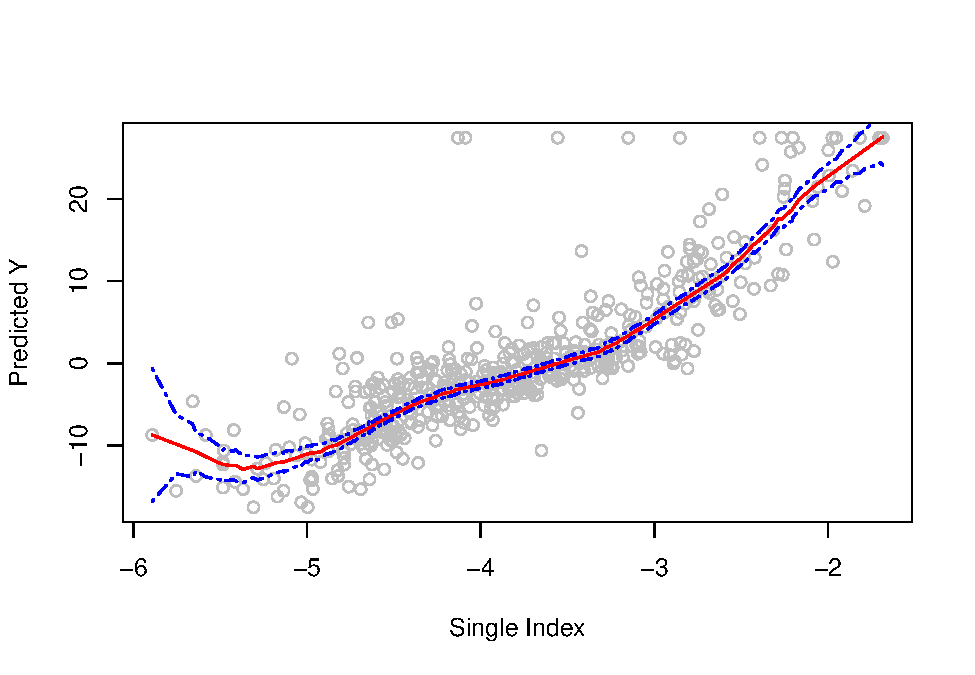
\includegraphics{siqr_files/figure-latex/unnamed-chunk-3-1} \end{Schunk}

\begin{Schunk}
\begin{Sinput}
plot.si(est,bootstrap_interval = TRUE)
\end{Sinput}

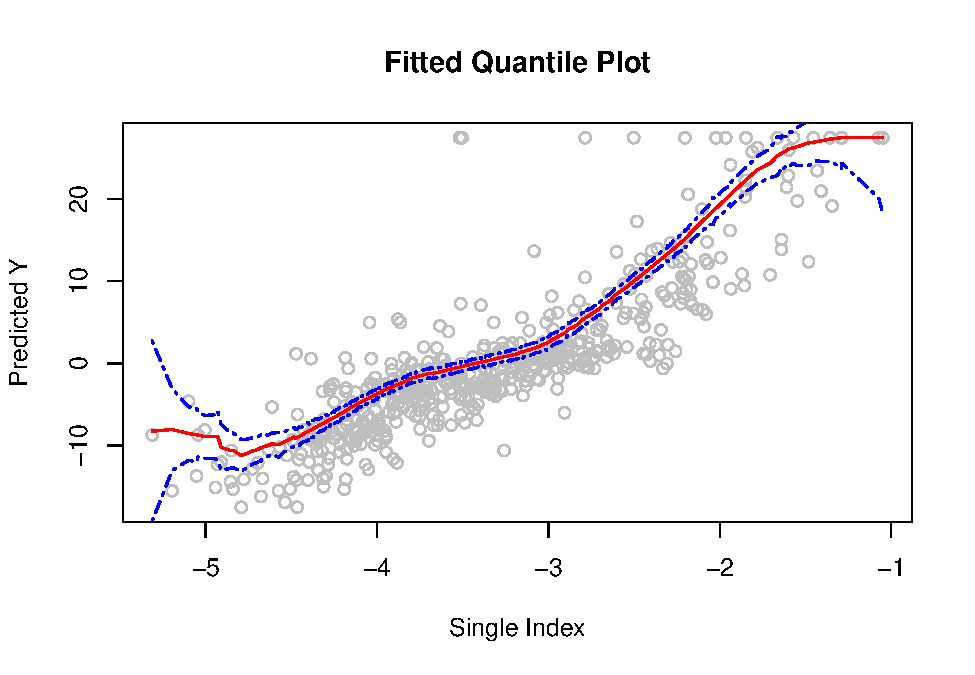
\includegraphics{siqr_files/figure-latex/unnamed-chunk-4-1} \end{Schunk}

\hypertarget{simulation}{%
\subsubsection{Simulation}\label{simulation}}

\begin{Schunk}
\begin{Sinput}
n <- 200
gamma0 <- c(1,2,3)
n_sim <- 100
p_vec <- c(0.1,0.25,0.5,0.75,0.9)

sim_results <- array(NA,dim = c(length(p_vec),ncol = 3,n_sim))
for(m in 1:n_sim){
  data <- generate_data(n)
  X <- data$X
  Y <- data$Y
  est.coefficient.sim <- matrix(NA, nrow = length(p_vec), ncol = NCOL(X))
  for (i in 1:length(p_vec)){
    est <- siqr(Y, X, gamma.inital = NULL, p=p_vec[i],maxiter = 30,tol = 1e-8)
    est.coefficient.sim[i,] <- est$gamma
  }
  sim_results[,,m] <- est.coefficient.sim
}
est.mean <- cbind(p_vec,apply(sim_results,c(1,2),mean))
colnames(est.mean) <- c("quantile tau","X1","X2","X3")
est.mean
\end{Sinput}
\end{Schunk}

\begin{Schunk}
\begin{Sinput}
#MC se
est.mean <- cbind(p_vec,apply(sim_results,c(1,2),sd))
colnames(est.mean) <- c("quantile tau","X1","X2","X3")
est.mean
\end{Sinput}
\end{Schunk}

\begin{Schunk}
\begin{Sinput}
Sys.sleep(100)
\end{Sinput}
\end{Schunk}

\bibliography{RJreferences}


\address{%
Author One\\
Affiliation\\
line 1\\ line 2\\
}
\href{mailto:author1@work}{\nolinkurl{author1@work}}

\address{%
Author Two\\
Affiliation\\
line 1\\ line 2\\
}
\href{mailto:author2@work}{\nolinkurl{author2@work}}

